\documentclass[12pt,a4paper]{article}
\usepackage{amsmath,amscd,amsbsy,amssymb,latexsym,url,bm,amsthm}
\usepackage{epsfig,graphicx,subfigure}
\usepackage{enumitem,balance}
\usepackage{wrapfig}
\usepackage{mathrsfs,euscript}
\usepackage[usenames]{xcolor}
\usepackage{hyperref}
\usepackage[vlined,ruled,linesnumbered]{algorithm2e}
\usepackage{array}
\usepackage{appendix}
\usepackage{soul}
\usepackage{listings}
\hypersetup{colorlinks=true,linkcolor=black}
\usepackage{attachfile}
\usepackage{listings}

\newtheorem{theorem}{Theorem}
\newtheorem{lemma}[theorem]{Lemma}
\newtheorem{proposition}[theorem]{Proposition}
\newtheorem{corollary}[theorem]{Corollary}
\newtheorem{exercise}{Exercise}
\newtheorem*{solution}{Solution}
\newtheorem{definition}{Definition}
\theoremstyle{definition}

\renewcommand{\thefootnote}{\fnsymbol{footnote}}

\newcommand{\postscript}[2]
 {\setlength{\epsfxsize}{#2\hsize}
  \centerline{\epsfbox{#1}}}

\renewcommand{\baselinestretch}{1.0}

\setlength{\oddsidemargin}{-0.365in}
\setlength{\evensidemargin}{-0.365in}
\setlength{\topmargin}{-0.3in}
\setlength{\headheight}{0in}
\setlength{\headsep}{0in}
\setlength{\textheight}{10.1in}
\setlength{\textwidth}{7in}
\makeatletter \renewenvironment{proof}[1][Proof] {\par\pushQED{\qed}\normalfont\topsep6\p@\@plus6\p@\relax\trivlist\item[\hskip\labelsep\bfseries#1\@addpunct{.}]\ignorespaces}{\popQED\endtrivlist\@endpefalse} \makeatother
\makeatletter
\renewenvironment{solution}[1][Solution] {\par\pushQED{\qed}\normalfont\topsep6\p@\@plus6\p@\relax\trivlist\item[\hskip\labelsep\bfseries#1\@addpunct{.}]\ignorespaces}{\popQED\endtrivlist\@endpefalse} \makeatother

\begin{document}
\noindent

%========================================================================
\noindent\framebox[\linewidth]{\shortstack[c]{
\Large{\textbf{Lab06-Linear Programming}}\vspace{1mm}\\
CS214-Algorithm and Complexity, Xiaofeng Gao, Spring 2021.}}
\begin{center}
\footnotesize{\color{blue}$*$ Name:\underline{\quad   Haoyi You  \quad  }\quad Student ID:\underline{\quad 519030910193 \quad} \quad Email: \underline{\quad yuri-you@sjtu.edu.cn \quad}}
\end{center}

\begin{enumerate}
    \item
    \textit{Hirschberg Algorithm.} Recall the \textbf{String Similarity} problem in class, in which we calculate the edit distance between two strings in a sequence alignment manner.
    \begin{enumerate}
    	\item
    	Implement the algorithm combining \textbf{dynamic programming} and \textbf{divide-and-conquer} strategy in C/C++. Analyze the time complexity of your algorithm. {\color{blue}(The template \emph{Code-SequenceAlignment.cpp} is attached on the course webpage)}.
    	    \begin{solution}
    \begin{enumerate}
       \item The code please refer to appendix 1.
       \item  Time Complexity:O(mn)\\
        Let $f(x,y)$ be the time complexity of the problem with $x$ words in $X$ and $y$ words in $Y$.\\
        In the algorithm, we divide the problem into two parts with $x$ and $\frac{y}{2}$.For each parts we separately use recursion and dynamic programming. So we can get the recursive formula:
        \begin{equation}
            f(x,y)=2*f(x,\frac{y}{2})+2*O(x*\frac{y}{2})
        \end{equation}
        Assume $f(x,y)\le cxy$.\\
        Firstly,when $y==2$ this is correct.\\
        Hypothesis:when $y<k$ is correct.\\
        When $y==k$,
        \begin{equation}
        f(x,k)\le 2*cx\frac{k}{2}+2*cx\frac{k}{2}=c*x*k
        \end{equation}
        So from the mathematical induction we get $f(x,y)=O(xy)$
    \end{enumerate}
    \end{solution}
    	\item
    	Given $\alpha(x, y) = |ascii(x) - acsii(y)|$, where $ascii(c)$ is the ASCII code of character $c$, and $\delta=13$. Find the edit distance between the following two strings.
    	\begin{align*}
    		X[1..60]=&\ CMQHZZRIQOQJOCFPRWOUXXCEMYSWUJ\\
    		&\ TAQBKAJIETSJPWUPMZLNLOMOZNLTLQ	
    	\end{align*}
    	\begin{align*}
    		Y[1..50]=&\ SUYLVMUSDROFBXUDCOHAATBKN\\
    		&\ AAENXEVWNLMYUQRPEOCJOCIMZ
    	\end{align*}
    	\begin{solution}
    	The answer is 385.The result please refer to figure~\ref{codesequence}. As for the previous output is too long to print in one figure, I adjust some of the '$endl$' to '$\backslash t$'.
    	\begin{figure}[htbp]
        \centering
        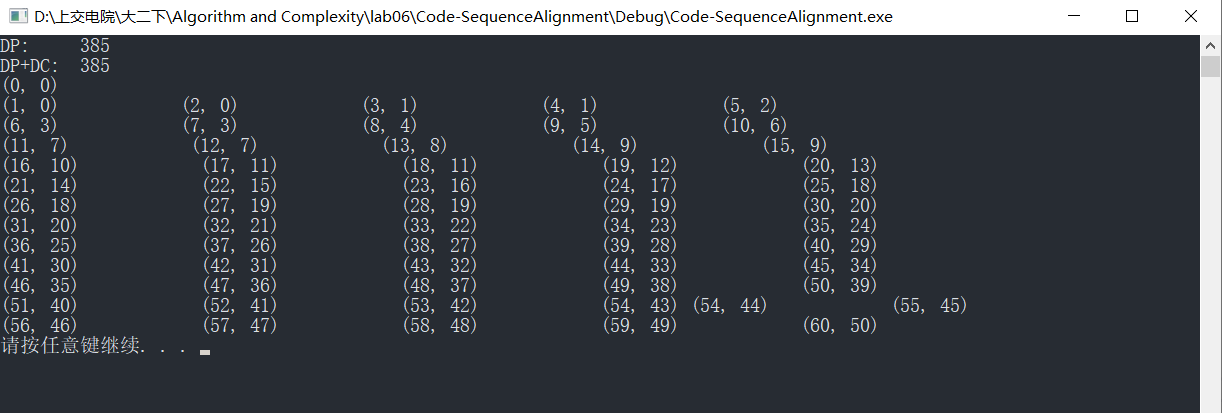
\includegraphics[width=0.9\textwidth]{Code-SequenceAlignment-result.png}
        \caption{Code SequenceAlignment output}\label{codesequence}
        \end{figure}
    	\end{solution}
    \end{enumerate}

    \item 
    \textit{Travelling Salesman Problem.} Given a list of cities and the distances between each pair of cities ($ G=(V,E,W) $), we want to find the shortest possible route that visits each city exactly once and returns to the origin city. Similar to \textbf{Maximum Independent Set} and '
    
    \textbf{Dominating Set}, please turn the traveling salesman problem into an ILP form.  
    
    \textbf{Remark:} $ W $ is the set of weights corresponds to the edges that connecting adjacent cities. \begin{solution}
    ~\par Suppose that $x_e$ is a 0-1 indicator of edge $e$, such that 
    \begin{equation}
        x_e=\left\{
    \begin{aligned}
    &1,~~e~is~selected~in~the~travelling~route \\
    &0,~~e~is~not~selected~in~the~travelling~route
    \end{aligned}
    \right.
    \end{equation}
    $\sum_{e\in E}x_e*w_e$ is the total length of the route, thus we can formulate the following \textbf{ILP}:\\
    \begin{equation}
    \begin{aligned}
        max~~~~~~&\sum_{e\in E}x_e*w_e\\
        \operatorname{s.t.}~~~~~~&x_e\in \{0,1\},~~~~~~~~\forall e\in E\\
        &d(v)=2, ~~~~~~~~~~~\forall v\in V\\
        \sum_{v\in V'}&d(v)<2*|V'|~~~~~~\forall V' \subset V\\
        with~~~~&d(v)=\sum_{e\in N(v)} x_e,~N(v)~is~the~total~edges~of~v\\
        \end{aligned}
    \end{equation}
    
    \end{solution}
    \item
    \textit{Investment Strategy.} A company intends to invest $0.3$ million yuan in $2021$, with a proper combination of the following $3$ projects:
    \begin{itemize}
    \item \textbf{Project 1:} Invest at the beginning of a year, and can receive a $20\%$ profit of the investment in this project at the end of this year. Both the capital and profit can be invested at the beginning of next year;
    \item \textbf{Project 2:} Invest at the beginning of $2021$, and can receive a $50\%$ profit of the investment in this project at the end of $2022$. The investment in this project cannot exceed $0.15$ million dollars;
    \item \textbf{Project 3:} Invest at the beginning of $2022$, and can receive a $40\%$ profit of the investment in this project at the end of $2022$. The investment in this project cannot exceed $0.1$ million dollars.
    \end{itemize}
    Assume that the company will invest \emph{all} its money at the beginning of a year. Please design a scheme of investment in $2021$ and $2022$ which maximizes the overall sum of capital and profit at the end of $2022$.
    \begin{enumerate}
    \item
    Formulate a linear programming with necessary explanations.

    \item
    Transform your LP into its standard form and slack form.

    \item
    Transform your LP into its dual form.

    \item
    Use the simplex method to solve your LP.
    \end{enumerate}
    \begin{solution}
        ~\par
    \begin{enumerate}
        \item Assume in 2021,the investment in Project 1 is $x_1$ and in Project 2 is $x_2$. In 2021, the investment in Project 1 is $x_3$ and in Project 3 is $x_4$.(unit: million dollars)
        \begin{enumerate}
        \item 
        Total sum of money $S=1.5*x_2+1.2*x_3+1.4*x_4$, the target is to maximize $S$
        \item 
        You cannot invest more money than you have, so there are 2 constrains in formula ~\ref{1}.\\
        \begin{equation}
            \label{1}
            \begin{aligned}
            x_1+x_2&\le 0.3\\
            x_3+x_4&\le 0.2*x_1+0.3-x_2 
            \end{aligned}
        \end{equation}
        \item 
        You cannot invest negative money. So there are\\
        \begin{equation}
            x_i\ge 0, i=1,2,3,4
        \end{equation}
        \end{enumerate}
        \item        
        \begin{enumerate}
            \item Stardard form:
            \begin{equation}
                \begin{aligned}
                maximize ~~~~~~~~~1.5x_2+1.2x_3+1&.4x_4\\
                \textbf{s.t. }~~~~~~~~~~~~~~~~~~~~~~x_1+x_2\le&~0.3\\
               -0.2x_1+x_2+x_3+x_4\le&~0.3\\
               x_2\le&~0.15\\
               x_4\le&~0.1\\
               x_1,x_2,x_3,x_4\ge&~0
                \end{aligned}
            \end{equation}
            \item Slack form:
            \begin{equation}
                \begin{aligned}
                maximize ~~~~~~~~~1.5x_2+1.2x_3+1&.4x_4\\
                \textbf{s.t. }~~~~~~~~~~~~~~~~x_1+x_2+s_1=&~0.3\\
               -0.2x_1+x_2+x_3+x_4+s_2=&~0.3\\
               x_2+s_3=&~0.15\\
               x_4+s_4=&~0.1\\
               x_1,x_2,x_3,x_4,s_1,s_2,s_3,s_4\ge&~0
                \end{aligned}
            \end{equation}
        \end{enumerate}
        \item Dual form:
         \begin{equation}
                \begin{aligned}
                minimize ~~~~~~~~~0.3y_1+0.3y_2+0.15y_3&+0.1y_4\\
                  \textbf{s.t. }~~~~~~~~~~~~~~~y_1+y_2+y_3\ge&~1.5\\
                y_1-0.2y_2\ge&~0\\
                y_2\ge&~1.2\\
                y_2+y_4\ge&~1.4\\
                y_1,y_2,y_3,y_4\ge&~0
                \end{aligned}
            \end{equation}
            \item 
            \begin{enumerate}
                \item Based on the slack form,let $(x_1,x_2,x_3,x_4,s_1,s_2,s_3,s_4)=(0,0,0,0,0.3,0.3,0.15,0.1)$
                \begin{equation}
                \begin{aligned}
                maximize ~~~~~~~~~1.5x_2+1.2x_3+1.4&x_4\\
                \textbf{s.t. }~~~~~~~~~~~~~~~~0.3-x_1-x_2=&~s_1\\
               0.3+0.2x_1-x_2-x_3-x_4=&~s_2\\
               0.15-x_2=&~s_3\\
               0.1-x_4=&~s_4\\
               x_1,x_2,x_3,x_4,s_1,s_2,&s_3,s_4\ge~0
                \end{aligned}
            \end{equation}
                \item Choose $x_4$,the limitation is 0.1, so we modify $S=1.5s_3+1.2x_3+1.4(0.1-s_4)$
                \item $(x_1,x_2,x_3,x_4,s_1,s_2,s_3,s_4)=(0,0,0,0.1,0.3,0.2,0.15,0)$ and change the equation 
            \begin{equation}
                \begin{aligned}
                maximize ~~~~~~~~~1.5x_2+1.2x_3+1.4&(0.1-s_4)\\
                \textbf{s.t. }~~~~~~~~~~~~~~~~0.3-x_1-x_2=&~s_1\\
               0.2+0.2x_1-x_2-x_3+s_4=&~s_2\\
               0.15-x_2=&~s_3\\
               0.1-s_4=&~x_4\\
               x_1,x_2,x_3,x_4,s_1,s_2,&s_3,s_4\ge~0
                \end{aligned}
            \end{equation}
                \item
                Choose $x_2$, the limitation is 0.15, so we modify $S=1.5(0.15-s_3)+1.2x_3+1.4(0.1-s_4)$
                \item $(x_1,x_2,x_3,x_4,s_1,s_2,s_3,s_4)=(0,0.15,0,0.1,0.15,0.05,0,0)$ and change the equation 
            \begin{equation}
                \begin{aligned}
                maximize ~~~~~~~~~1.5(0.15-s_3)+1.2x_3+1.4(0.1-s_4)\\
                \textbf{s.t. }~~~~~~~~~~~~~~~~0.15+s_3-x_1=&~s_1\\
               0.05+0.2x_1-x_3+s_4+s_3=&~s_2\\
               0.15-s_3=&~x_2\\
               0.1-s_4=&~x_4\\
               x_1,x_2,x_3,x_4,s_1,s_2,&s_3,s_4\ge~0
                \end{aligned}
            \end{equation}
            \item
                Choose $x_3$, the limitation is 0.05, so we modify $S=1.5(0.15-s_3)+1.2(0.05-s_2+0.2x_1+s_4+s_3)+1.4(0.1-s_4)=0.425+0.24x_1-1.2s_2-0.3s_3-0.2s_4$
                \item $(x_1,x_2,x_3,x_4,s_1,s_2,s_3,s_4)=(0,0.15,0.05,0.1,0.15,0,0,0)$ and change the equation 
            \begin{equation}
                \begin{aligned}
                maximize ~~~~~~~~~0.425+0.24x_1-1.2s_2-0.3s_3-0.2s_4\\
                \textbf{s.t. }~~~~~~~~~~~~~~~~0.15+s_3-x_1=&~s_1\\
               0.05+0.2x_1-s_3+s_4+s_3=&~x_3\\
               0.15-s_3=&~x_2\\
               0.1-s_4=&~x_4\\
               x_1,x_2,x_3,x_4,s_1,s_2,&s_3,s_4\ge~0
                \end{aligned}
            \end{equation}
            \item
                Choose $x_1$, the limitation is 0.15, so we modify $S=0.461-0.24s_1-0.06s_3-1.2s_2-0.2s_4$
                \item $(x_1,x_2,x_3,x_4,s_1,s_2,s_3,s_4)=(0.15,0.15,0.08,0.1,0,0,0,0)$
                \item Here there are no positive valuable in target. So the total sum is 0.461.
            \end{enumerate}
    \end{enumerate}    
    \end{solution}
    \item
    \textit{Factory Production.} An engineering factory makes seven products (PROD 1 to PROD 7) on the following machines: four grinders, two vertical drills, three horizontal drills, one borer and one planer. Each product yields a certain contribution to profit (in \pounds/unit). These quantities (in \pounds/unit) together with the unit production times (hours) required on each process are given below. A dash indicates that a product does not require a process.

    \begin{table}[htbp]
      \scriptsize
      \centering
      \renewcommand\arraystretch{1.1}
      \begin{tabular}{m{0.18\textwidth} m{0.07\textwidth}<{\centering} m{0.07\textwidth}<{\centering} m{0.07\textwidth}<{\centering} m{0.07\textwidth}<{\centering} m{0.07\textwidth}<{\centering} m{0.07\textwidth}<{\centering} m{0.07\textwidth}<{\centering}}
      \hline
       & \textbf{PROD 1} & \textbf{PROD 2} & \textbf{PROD 3} & \textbf{PROD 4} & \textbf{PROD 5} & \textbf{PROD 6} &  \textbf{PROD 7} \\\hline
      Contribution to profit & 10 & 6 & 8 & 4 & 11 & 9 & 3 \\
      Grinding & 0.5 & 0.7 & - & - & 0.3 & 0.2 & 0.5 \\
      Vertical drilling & 0.1 & 0.2 & - & 0.3 & - & 0.6 & - \\
      Horizontal drilling & 0.2 & - & 0.8 & - & - & - & 0.6 \\
      Boring & 0.05 & 0.03 & - & 0.07 & 0.1 & - & 0.08 \\
      Planing & - & - & 0.01 & - & 0.05 & - & 0.05 \\
      \hline
      \end{tabular}
    \end{table}

    There are marketing limitations on each product in each month, given in the following table:

    \begin{table}[htbp]
      \scriptsize
      \centering
      \renewcommand\arraystretch{1.1}
      \begin{tabular}{m{0.1\textwidth} m{0.07\textwidth}<{\centering} m{0.07\textwidth}<{\centering} m{0.07\textwidth}<{\centering} m{0.07\textwidth}<{\centering} m{0.07\textwidth}<{\centering} m{0.07\textwidth}<{\centering} m{0.07\textwidth}<{\centering}}
      \hline
       & \textbf{PROD 1} & \textbf{PROD 2} & \textbf{PROD 3} & \textbf{PROD 4} & \textbf{PROD 5} & \textbf{PROD 6} &  \textbf{PROD 7} \\\hline
      January & 500 & 1000 & 300 & 300 & 800 & 200 & 100 \\
      February & 600 & 500 & 200 & 0 & 400 & 300 & 150 \\
      March & 300 & 600 & 0 & 0 & 500 & 400 & 100 \\
      April & 200 & 300 & 400 & 500 & 200 & 0 & 100 \\
      May & 0 & 100 & 500 & 100 & 1000 & 300 & 0 \\
      June & 500 & 500 & 100 & 300 & 1100 & 500 & 60 \\
      \hline
      \end{tabular}
    \end{table}

    It is possible to store up to 100 of each product at a time at a cost of \pounds0.5 per unit per month (charged at the end of each month according to the amount held at that time). There are no stocks at present, but it is desired to have a stock of exactly 50 of each type of product at the end of June. The factory works six days a week with two shifts of 8h each day. It may be assumed that each month consists of only 24 working days. Each machine must be down for maintenance in one month of the six. No sequencing problems need to be considered.

    When and what should the factory make in order to maximize the total net profit?

    \begin{enumerate}
    \item
    Use \emph{CPLEX Optimization Studio} to solve this problem. Describe your model in \emph{Optimization Programming Language} (OPL). Remember to use a separate data file (.dat) rather than embedding the data into the model file (.mod).

    \item
    Solve your model and give the following results.
    \begin{enumerate}
    \item
    For each machine:
    \begin{enumerate}
    \item
    the month for maintenance.
    \end{enumerate}
    \item
    For each product:
    \begin{enumerate}
    \item
    The amount to make in each month.
    \item
    The amount to sell in each month.
    \item
    The amount to hold at the end of each month.
    \end{enumerate}
    \item
    The total selling profit.
    \item
    The total holding cost.
    \item
    The total net profit (selling profit minus holding cost).
    \end{enumerate}
    \end{enumerate}
    \begin{solution}
    \begin{enumerate}
        
    \item Please refer to appendix 3.
    
    \item Please refer to figure ~\ref{factory}
    \begin{figure}[htbp]
        \centering
        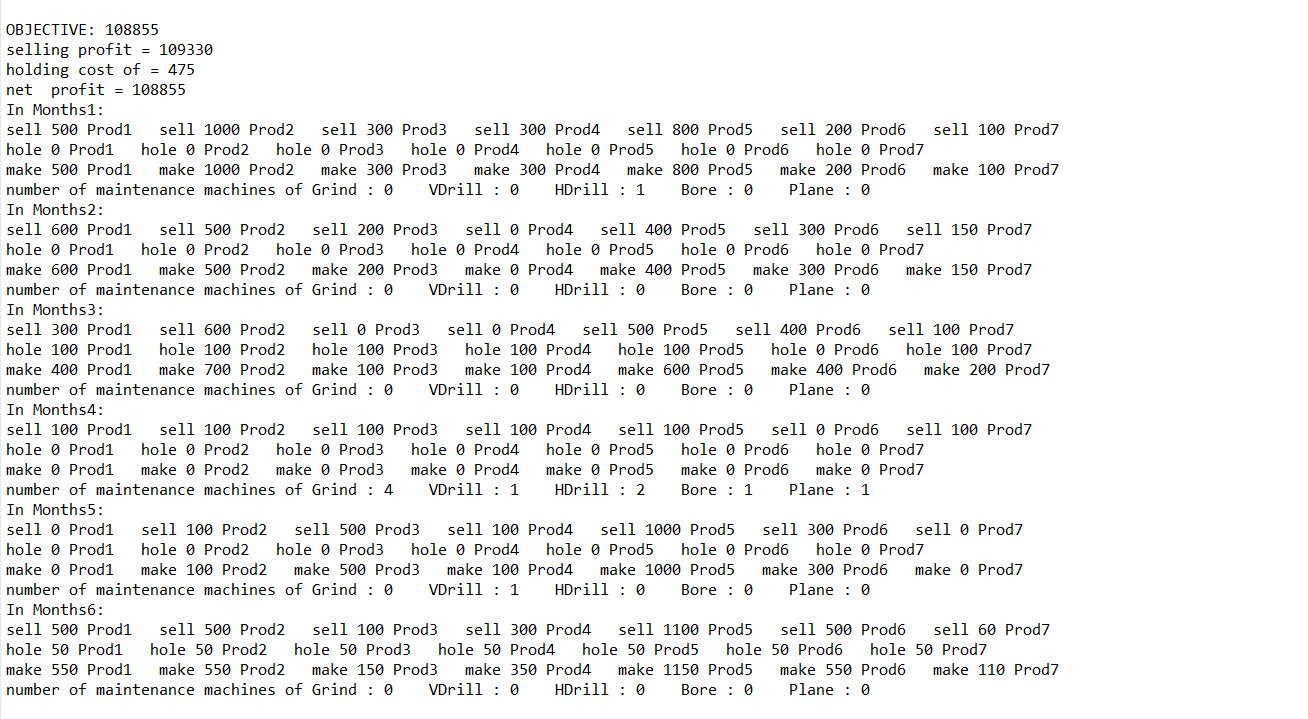
\includegraphics[width=1.2\textwidth]{factory.png}
        \caption{Factory Production linear solution}\label{factory}
        \end{figure}
    \end{enumerate}
    
    \end{solution}

\end{enumerate}
\newpage
\vspace{20pt}

{\noindent\large\textbf{Appendix 1}}
\begin{enumerate}
	\item [\textbf{A.}]
	\textbf{FactoryPlanning.dat}
	\attachfile{FactoryPlanning.dat}
	\lstset{
		language=C,
		tabsize=2,
		basicstyle=\footnotesize\ttfamily,
		columns=fullflexible,
		keywordstyle=\color{blue},
		numbers=left,
		numberstyle=\scriptsize\ttfamily,
		frame=single
	}
	\begin{lstlisting}
		NbMonths = 6;
		
		Prod = {Prod1, Prod2, Prod3, Prod4, Prod5, Prod6, Prod7};
		Process = {Grind, VDrill, HDrill, Bore, Plane};
		
		// profitProd[j] is profit per unit for product j
		ProfitProd = [10 6 8 4 11 9 3];
		
		// processProd[i][j] gives hours of process i required by product j
		ProcessProd = [[0.5  0.7  0.0  0.0  0.3  0.2 0.5 ]
		[0.1  0.2  0.0  0.3  0.0  0.6 0.0 ]
		[0.2  0.0  0.8  0.0  0.0  0.0 0.6 ]
		[0.05 0.03 0.0  0.07 0.1  0.0 0.08]
		[0.0  0.0  0.01 0.0  0.05 0.0 0.05]];
		
		// marketProd[i][j] gives marketing limitation on product j for month i
		MarketProd = [[500 1000 300  300 800  200 100]
		[600 500  200  0   400  300 150]
		[300 600  0    0   500  400 100]
		[200 300  400  500 200  0   100]
		[0   100  500  100 1000 300 0  ]
		[500 500  100  300 1100 500 60 ]];
		
		CostHold  = 0.5;
		StartHold = 0;
		EndHold   = 50;
		MaxHold   = 100;
		
		// process capacity
		HoursMonth = 384; // 2 eight hour shifts per day, 24 working days per month;
		
		// number of each type of machine
		NumProcess = [4 2 3 1 1];
		
		// how many machines must be down over 6 month period
		NumDown = [4 2 3 1 1];
	\end{lstlisting}
\end{enumerate}

\appendix
\noindent\large\textbf{Appendix 3}
\begin{lstlisting}[numberstyle=\tiny, 
        basicstyle=\small]

{string} Prod = ...;
{string} Process = ...;

int NbMonths = ...;
range Months=1..NbMonths;
float ProfitProd[Prod]=...;
float ProcessProd[Process][Prod]= ...;
int MarketProd[Months][Prod] = ...;

float CostHold = ...;
int StartHold = ...;
int EndHold = ...;
int MaxHold = ...;

int HoursMonth = ...;

int NumProcess[Process] = ...;
int NumDown[Process] = ...;
dvar int+ product[Months][Prod];
dvar int+ produce[Months][Prod];
dvar int+ sell[Months][Prod];
dvar int+ remain[Months][Prod];
dvar int+ down[Months][Process];
dvar float+ Profit;
dvar float+ Cost;
maximize Profit-Cost;
subject to{
	/*relationship constrain*/
	forall(i in Prod){
		forall(j in Months){
		  	remain[j][i]==product[j][i]-sell[j][i];
  		 }		  	
	}
	forall(i in Months){
		forall(j in Prod){
			sell[i][j]<=MarketProd[i][j];		
		}	
	}
	forall(i in Months){
		forall(j in Prod){
			if(i==1){
				product[i][j]==produce[i][j]+StartHold;			
			}		
			else{
				product[i][j]==produce[i][j]+remain[i-1][j];	
			}
		}	
	}
	
	/*machine down constrain*/
	forall(j in Process){
		sum(i in Months)down[i][j] == NumDown[j];
	}
	
	/*produce machine constarin */
	forall(i in Months){
		forall(j in Process){
			sum(k in Prod)(produce[i][k]*ProcessProd[j][k])<=HoursMonth
			*(NumProcess[j]-down[i][j]);
		}
	}
	/*store constrain*/
	forall(i in Months){
		forall(j in Prod){
			if(i==NbMonths){
				remain[i][j]==EndHold;		
			}	
			else{
				remain[i][j]<=MaxHold;			
			}
		}
	}
	Profit == sum(i in Months) sum(j in Prod)sell[i][j]*ProfitProd[j];
	Cost == sum(i in 1..NbMonths)sum(j in Prod)remain[i][j]*CostHold;
}
execute {
	if (cplex.getCplexStatus() == 1) {
    	writeln('selling profit = ', Profit)
    	writeln('holding cost of = ', Cost)
    	writeln('net  profit = ', Profit-Cost)
		for(i in Months){
			write('In Months',i)		
			write(':\n')
			for(j in Prod)	{
				write("sell ",sell[i][j])
				write(" ",j)
				write("   ")	
  			}
  			write("\n")		
  			for(j in Prod)	{
				write("hole ",remain[i][j])
				write(" ",j)
				write("   ")	
  			}
  			write("\n")		
  			for(j in Prod)	{
				write("make ",produce[i][j])
				write(" ",j)
				write("   ")	
  			}
  			write("\n")	
  			write("number of maintenance machines of ")
  			for(j in Process)	{
				write(j)
				write(" : ",down[i][j])
				write("    ")
  			}
  			write("\n")					
		}
	}
}

\end{lstlisting}

%========================================================================
\end{document}
